\documentclass[12pt,a4paper]{article}
\usepackage{preamble}
\let\AltKey=\Alt
\let\Alt=\relax
\usepackage{menukeys}
\newcommand\sessiontitle{Lab Session 1}
\newcommand\sessionsubtitle{Python introduction and Jupyter notebooks}

%%%%%%%%%%%%%%%%%%%%%%%%%%%%%%%%%%%%%%%%%%
\begin{document}

\begin{description}
\item[Course web-page:] \begin{sloppypar}\url{http://www.bioquant.uni-heidelberg.de/research/groups/biomedical-computer-vision/teaching/compmeth/Labsessions}\end{sloppypar}
\item[Opening a terminal on macOS:] Simultaneously press \keystroke{\cmd}+\Spacebar to bring up Spotlight, type ``terminal'', then press \Return.
\item[Opening a terminal on Linux:] Simultaneously press \Ctrl+\AltKey+\keystroke{T}.
\end{description}

\section{Preparation}
\label{task:preparation}
\begin{enumerate}
\item Mamba is a fast and reliable tool for installation of Conda packages. Mambaforge is a Conda distribution which comes with Mamba out-of-the-box.
    \begin{description}
        \item[If you have no Conda distribution installed yet,] download and install Mamba\-forge from: \url{https://github.com/conda-forge/miniforge#mambaforge}
        \begin{description}
            \item[Installation on Windows:] Run the downloaded file. If Windows complains that this is a risky action since the source of the file is unknown, click ``More info'' and then ``Run anyway''. Leave all options on default.
            \item[Installation on macOS and Linux:] Open a terminal. Inside the terminal, type ``\texttt{cd Downloads}'' and press \Return to change the current directory to where your Downloads are stored by default. Make the downloaded file runnable by typing ``\texttt{chmod +x Mambaforge-*.sh}'' and pressing \Return. Run the downloaded file by typing ``\texttt{sh Mambaforge-*.sh}'' and pressing \Return. Follow the on-screen instructions. When the license is shown, press \Spacebar to turn pages. You will be asked a yes/no-question twice, type ``\texttt{yes}'' both times, and leave all other options on default. When you see the text ``Thank you for installing Mambaforge!'', the installation is finished, and you should close the terminal.
        \end{description}
        \item[If you already have Mamba installed on your computer,] proceed to Step~2.
        \item[Otherwise,] install the package ``mamba'' in the ``base'' environment of your Conda distribution, as explained here: \url{https://mamba.readthedocs.io/en/latest/installation.html#existing-conda-install} -- ask a supervisor if you need assistance.
    \end{description}
\item Download the course material from the course web-page.
\item Extract the downloaded course material ZIP file \emph{\underline{\smash{directly}} into your \underline{\smash{Home directory}}}. \underline{\smash{\textbf{\emph{Double-check this!}}}} For example, \textbf{on Windows}, you can find your Home directory by navigating to \texttt{\%userprofile\%} in Explorer:\\[0.5em]
    \begin{minipage}{\linewidth}
        \centering
        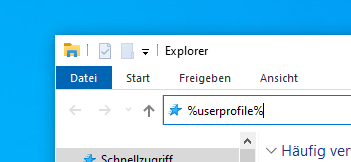
\includegraphics[height=35mm]{images/userprofile.png}
    \end{minipage}
    
    After extraction of the course material ZIP file, your Home directory is supposed to look as shown on the left below, and \underline{\smash{\emph{not}}} as shown on the right:\\[0.5em]
    \begin{minipage}{\linewidth}
        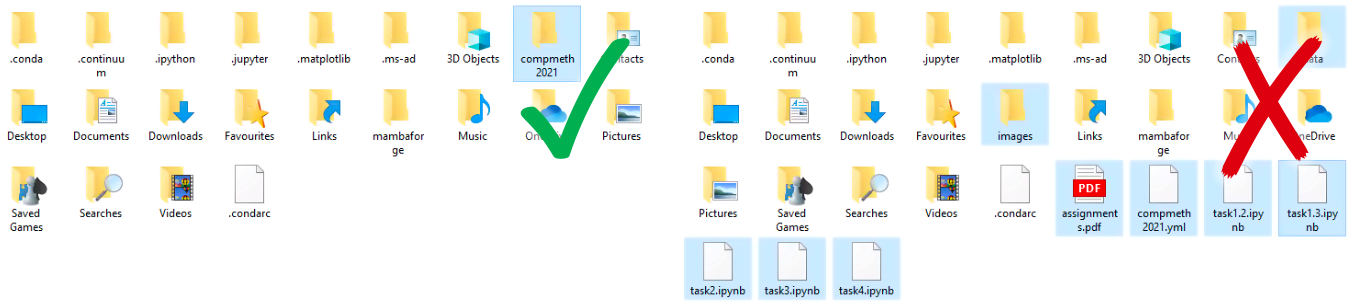
\includegraphics[width=\linewidth]{images/course-material.png}
    \end{minipage}\\

    \textbf{On macOS,} you will usually find the already extracted ``\texttt{{\projectid}}'' directory in your Downloads directory, immediately after the download of the course material is finished. The best practice then is to simply drag the ``\texttt{{\projectid}}'' directory from your Downloads directory to your Home directory in Finder. To find the directories in Finder, simultaneously press \keystroke{\Alt}+\keystroke{\cmd}+\keystroke{L} for the Downloads directory, and \keystroke{\shift}+\keystroke{\cmd}+\keystroke{H} for the Home directory. 
\item Import the Conda environment as follows:
    \begin{enumerate}
        \item Open a prompt or terminal, depending on your operating system:
        \begin{description}
            \item[On Windows:] Run the ``Miniforge Prompt'' from your Start Menu.
            \item[On macOS and Linux:] Open a terminal. It is important that you open a \emph{new} terminal here (do \emph{not} use the terminal you used for Step~1).
        \end{description}
        \item Inside the prompt/terminal, type: ``\texttt{cd {\projectid}}'' and press \Return to change into the directory where you had extracted the course material before.
        \item Type ``\texttt{mamba env create -f {\ymlfile}}'', then press \Return to start the import procedure.
    \end{enumerate}
    
    Depending on the bandwidth of your internet connection, the import procedure might take several minutes. You may close the prompt/terminal afterwards.
\end{enumerate}

\section{Your first Jupyter notebook}
The assignments of this course are organized into several Jupyter notebooks. They are included into the course material ZIP file you downloaded before. By progressing from task to task, you will have to work with different notebooks, so it is important that you know how to open them.

To open your first notebook, proceed as follows:
\begin{enumerate}
    \item Run the ``Miniforge Prompt'' or open a terminal (depending on your operating system, as you did in Task~\ref{task:preparation}, Step~4a).
    \item Inside the prompt/terminal, type: ``\texttt{cd {\projectid}}'' and press \Return to change into the course material directory (as you did in Task~\ref{task:preparation}, Step~4b).
    \item Type ``\texttt{conda activate {\projectid}}'' and press \Return to activate the Conda environment you imported before.
    \item Type ``\texttt{jupyter notebook task1.2.ipynb}'' and press \Return. Wait a few seconds and you will see that a browser window opens.
    \item Follow the on-screen instructions -- \textbf{Note:} Jupyter permits running code cells and Markdown cells in an \emph{arbitrary order}. This is very helpful for experimenting and trying out new things. \textbf{Nevertheless, an assignment in this course is \emph{only} considered ``finished'' when the results can be reproduced by re-running all code cells \emph{from top to bottom}!} You can check this easily by choosing ``Restart \& Run All'' from the ``Kernel'' menu of an opened Jupyter notebook.
    \item When finished, save your notebook (menu ``File'', then ``Save and Checkpoint'') and close the notebook (menu ``File'', then ``Close and Halt'').
    \item The last step is to shut down the notebook server: Return to your console/terminal and simultaneously press \Ctrl+\keystroke{C}. If asked to confirm the shutdown of the notebook server, press \keystroke{Y}\Return subsequently. You may now close the console/terminal.
\end{enumerate}
Note that the order of the Steps~2 and~3 is interchangeable.

\section{Writing loops in Python}
Now you already know how to open, save, and close a Jupyter notebook.
\begin{enumerate}
    \item Return to your prompt/terminal. If you had closed it before, re-open it and change into the course material directory (use ``\texttt{cd {\projectid}}'' as described above), and activate the Conda environment (use ``\texttt{conda activate {\projectid}}'' as described above).
    \item Open the Jupyter notebook \texttt{task1.3.ipynb} and follow the on-screen instructions (use ``\texttt{jupyter notebook task1.3.ipynb}'' as described above).
    \item Save your notebook and shut down the notebook server (as described above).
\end{enumerate}
\end{document}
